% Options for packages loaded elsewhere
% Options for packages loaded elsewhere
\PassOptionsToPackage{unicode}{hyperref}
\PassOptionsToPackage{hyphens}{url}
\PassOptionsToPackage{dvipsnames,svgnames,x11names}{xcolor}
%
\documentclass[
  letterpaper,
  DIV=11,
  numbers=noendperiod]{scrartcl}
\usepackage{xcolor}
\usepackage{amsmath,amssymb}
\setcounter{secnumdepth}{5}
\usepackage{iftex}
\ifPDFTeX
  \usepackage[T1]{fontenc}
  \usepackage[utf8]{inputenc}
  \usepackage{textcomp} % provide euro and other symbols
\else % if luatex or xetex
  \usepackage{unicode-math} % this also loads fontspec
  \defaultfontfeatures{Scale=MatchLowercase}
  \defaultfontfeatures[\rmfamily]{Ligatures=TeX,Scale=1}
\fi
\usepackage{lmodern}
\ifPDFTeX\else
  % xetex/luatex font selection
\fi
% Use upquote if available, for straight quotes in verbatim environments
\IfFileExists{upquote.sty}{\usepackage{upquote}}{}
\IfFileExists{microtype.sty}{% use microtype if available
  \usepackage[]{microtype}
  \UseMicrotypeSet[protrusion]{basicmath} % disable protrusion for tt fonts
}{}
\makeatletter
\@ifundefined{KOMAClassName}{% if non-KOMA class
  \IfFileExists{parskip.sty}{%
    \usepackage{parskip}
  }{% else
    \setlength{\parindent}{0pt}
    \setlength{\parskip}{6pt plus 2pt minus 1pt}}
}{% if KOMA class
  \KOMAoptions{parskip=half}}
\makeatother
% Make \paragraph and \subparagraph free-standing
\makeatletter
\ifx\paragraph\undefined\else
  \let\oldparagraph\paragraph
  \renewcommand{\paragraph}{
    \@ifstar
      \xxxParagraphStar
      \xxxParagraphNoStar
  }
  \newcommand{\xxxParagraphStar}[1]{\oldparagraph*{#1}\mbox{}}
  \newcommand{\xxxParagraphNoStar}[1]{\oldparagraph{#1}\mbox{}}
\fi
\ifx\subparagraph\undefined\else
  \let\oldsubparagraph\subparagraph
  \renewcommand{\subparagraph}{
    \@ifstar
      \xxxSubParagraphStar
      \xxxSubParagraphNoStar
  }
  \newcommand{\xxxSubParagraphStar}[1]{\oldsubparagraph*{#1}\mbox{}}
  \newcommand{\xxxSubParagraphNoStar}[1]{\oldsubparagraph{#1}\mbox{}}
\fi
\makeatother

\usepackage{color}
\usepackage{fancyvrb}
\newcommand{\VerbBar}{|}
\newcommand{\VERB}{\Verb[commandchars=\\\{\}]}
\DefineVerbatimEnvironment{Highlighting}{Verbatim}{commandchars=\\\{\}}
% Add ',fontsize=\small' for more characters per line
\usepackage{framed}
\definecolor{shadecolor}{RGB}{241,243,245}
\newenvironment{Shaded}{\begin{snugshade}}{\end{snugshade}}
\newcommand{\AlertTok}[1]{\textcolor[rgb]{0.68,0.00,0.00}{#1}}
\newcommand{\AnnotationTok}[1]{\textcolor[rgb]{0.37,0.37,0.37}{#1}}
\newcommand{\AttributeTok}[1]{\textcolor[rgb]{0.40,0.45,0.13}{#1}}
\newcommand{\BaseNTok}[1]{\textcolor[rgb]{0.68,0.00,0.00}{#1}}
\newcommand{\BuiltInTok}[1]{\textcolor[rgb]{0.00,0.23,0.31}{#1}}
\newcommand{\CharTok}[1]{\textcolor[rgb]{0.13,0.47,0.30}{#1}}
\newcommand{\CommentTok}[1]{\textcolor[rgb]{0.37,0.37,0.37}{#1}}
\newcommand{\CommentVarTok}[1]{\textcolor[rgb]{0.37,0.37,0.37}{\textit{#1}}}
\newcommand{\ConstantTok}[1]{\textcolor[rgb]{0.56,0.35,0.01}{#1}}
\newcommand{\ControlFlowTok}[1]{\textcolor[rgb]{0.00,0.23,0.31}{\textbf{#1}}}
\newcommand{\DataTypeTok}[1]{\textcolor[rgb]{0.68,0.00,0.00}{#1}}
\newcommand{\DecValTok}[1]{\textcolor[rgb]{0.68,0.00,0.00}{#1}}
\newcommand{\DocumentationTok}[1]{\textcolor[rgb]{0.37,0.37,0.37}{\textit{#1}}}
\newcommand{\ErrorTok}[1]{\textcolor[rgb]{0.68,0.00,0.00}{#1}}
\newcommand{\ExtensionTok}[1]{\textcolor[rgb]{0.00,0.23,0.31}{#1}}
\newcommand{\FloatTok}[1]{\textcolor[rgb]{0.68,0.00,0.00}{#1}}
\newcommand{\FunctionTok}[1]{\textcolor[rgb]{0.28,0.35,0.67}{#1}}
\newcommand{\ImportTok}[1]{\textcolor[rgb]{0.00,0.46,0.62}{#1}}
\newcommand{\InformationTok}[1]{\textcolor[rgb]{0.37,0.37,0.37}{#1}}
\newcommand{\KeywordTok}[1]{\textcolor[rgb]{0.00,0.23,0.31}{\textbf{#1}}}
\newcommand{\NormalTok}[1]{\textcolor[rgb]{0.00,0.23,0.31}{#1}}
\newcommand{\OperatorTok}[1]{\textcolor[rgb]{0.37,0.37,0.37}{#1}}
\newcommand{\OtherTok}[1]{\textcolor[rgb]{0.00,0.23,0.31}{#1}}
\newcommand{\PreprocessorTok}[1]{\textcolor[rgb]{0.68,0.00,0.00}{#1}}
\newcommand{\RegionMarkerTok}[1]{\textcolor[rgb]{0.00,0.23,0.31}{#1}}
\newcommand{\SpecialCharTok}[1]{\textcolor[rgb]{0.37,0.37,0.37}{#1}}
\newcommand{\SpecialStringTok}[1]{\textcolor[rgb]{0.13,0.47,0.30}{#1}}
\newcommand{\StringTok}[1]{\textcolor[rgb]{0.13,0.47,0.30}{#1}}
\newcommand{\VariableTok}[1]{\textcolor[rgb]{0.07,0.07,0.07}{#1}}
\newcommand{\VerbatimStringTok}[1]{\textcolor[rgb]{0.13,0.47,0.30}{#1}}
\newcommand{\WarningTok}[1]{\textcolor[rgb]{0.37,0.37,0.37}{\textit{#1}}}

\usepackage{longtable,booktabs,array}
\usepackage{calc} % for calculating minipage widths
% Correct order of tables after \paragraph or \subparagraph
\usepackage{etoolbox}
\makeatletter
\patchcmd\longtable{\par}{\if@noskipsec\mbox{}\fi\par}{}{}
\makeatother
% Allow footnotes in longtable head/foot
\IfFileExists{footnotehyper.sty}{\usepackage{footnotehyper}}{\usepackage{footnote}}
\makesavenoteenv{longtable}
\usepackage{graphicx}
\makeatletter
\newsavebox\pandoc@box
\newcommand*\pandocbounded[1]{% scales image to fit in text height/width
  \sbox\pandoc@box{#1}%
  \Gscale@div\@tempa{\textheight}{\dimexpr\ht\pandoc@box+\dp\pandoc@box\relax}%
  \Gscale@div\@tempb{\linewidth}{\wd\pandoc@box}%
  \ifdim\@tempb\p@<\@tempa\p@\let\@tempa\@tempb\fi% select the smaller of both
  \ifdim\@tempa\p@<\p@\scalebox{\@tempa}{\usebox\pandoc@box}%
  \else\usebox{\pandoc@box}%
  \fi%
}
% Set default figure placement to htbp
\def\fps@figure{htbp}
\makeatother





\setlength{\emergencystretch}{3em} % prevent overfull lines

\providecommand{\tightlist}{%
  \setlength{\itemsep}{0pt}\setlength{\parskip}{0pt}}



 


\KOMAoption{captions}{tableheading}
\makeatletter
\@ifpackageloaded{tcolorbox}{}{\usepackage[skins,breakable]{tcolorbox}}
\@ifpackageloaded{fontawesome5}{}{\usepackage{fontawesome5}}
\definecolor{quarto-callout-color}{HTML}{909090}
\definecolor{quarto-callout-note-color}{HTML}{0758E5}
\definecolor{quarto-callout-important-color}{HTML}{CC1914}
\definecolor{quarto-callout-warning-color}{HTML}{EB9113}
\definecolor{quarto-callout-tip-color}{HTML}{00A047}
\definecolor{quarto-callout-caution-color}{HTML}{FC5300}
\definecolor{quarto-callout-color-frame}{HTML}{acacac}
\definecolor{quarto-callout-note-color-frame}{HTML}{4582ec}
\definecolor{quarto-callout-important-color-frame}{HTML}{d9534f}
\definecolor{quarto-callout-warning-color-frame}{HTML}{f0ad4e}
\definecolor{quarto-callout-tip-color-frame}{HTML}{02b875}
\definecolor{quarto-callout-caution-color-frame}{HTML}{fd7e14}
\makeatother
\makeatletter
\@ifpackageloaded{caption}{}{\usepackage{caption}}
\AtBeginDocument{%
\ifdefined\contentsname
  \renewcommand*\contentsname{Table of contents}
\else
  \newcommand\contentsname{Table of contents}
\fi
\ifdefined\listfigurename
  \renewcommand*\listfigurename{List of Figures}
\else
  \newcommand\listfigurename{List of Figures}
\fi
\ifdefined\listtablename
  \renewcommand*\listtablename{List of Tables}
\else
  \newcommand\listtablename{List of Tables}
\fi
\ifdefined\figurename
  \renewcommand*\figurename{Figure}
\else
  \newcommand\figurename{Figure}
\fi
\ifdefined\tablename
  \renewcommand*\tablename{Table}
\else
  \newcommand\tablename{Table}
\fi
}
\@ifpackageloaded{float}{}{\usepackage{float}}
\floatstyle{ruled}
\@ifundefined{c@chapter}{\newfloat{codelisting}{h}{lop}}{\newfloat{codelisting}{h}{lop}[chapter]}
\floatname{codelisting}{Listing}
\newcommand*\listoflistings{\listof{codelisting}{List of Listings}}
\makeatother
\makeatletter
\makeatother
\makeatletter
\@ifpackageloaded{caption}{}{\usepackage{caption}}
\@ifpackageloaded{subcaption}{}{\usepackage{subcaption}}
\makeatother
\usepackage{bookmark}
\IfFileExists{xurl.sty}{\usepackage{xurl}}{} % add URL line breaks if available
\urlstyle{same}
\hypersetup{
  pdftitle={Decision Tree Challenge},
  colorlinks=true,
  linkcolor={blue},
  filecolor={Maroon},
  citecolor={Blue},
  urlcolor={Blue},
  pdfcreator={LaTeX via pandoc}}


\title{Decision Tree Challenge}
\usepackage{etoolbox}
\makeatletter
\providecommand{\subtitle}[1]{% add subtitle to \maketitle
  \apptocmd{\@title}{\par {\large #1 \par}}{}{}
}
\makeatother
\subtitle{Feature Importance and Categorical Variable Encoding}
\author{}
\date{}
\begin{document}
\maketitle


\section{🌳 Decision Tree Challenge - Feature Importance and Variable
Encoding}\label{decision-tree-challenge---feature-importance-and-variable-encoding}

\subsection{Challenge Overview}\label{challenge-overview}

\textbf{Your Mission:} Create a simple GitHub Pages site that
demonstrates how decision trees measure feature importance and analyzes
the critical differences between categorical and numerical variable
encoding. You'll answer two key discussion questions by adding narrative
to a pre-built analysis and posting those answers to your GitHub Pages
site as a rendered HTML document.

\begin{tcolorbox}[enhanced jigsaw, breakable, opacityback=0, titlerule=0mm, colbacktitle=quarto-callout-warning-color!10!white, opacitybacktitle=0.6, arc=.35mm, left=2mm, colframe=quarto-callout-warning-color-frame, bottomtitle=1mm, toptitle=1mm, title=\textcolor{quarto-callout-warning-color}{\faExclamationTriangle}\hspace{0.5em}{⚠️ AI Partnership Required}, coltitle=black, rightrule=.15mm, leftrule=.75mm, toprule=.15mm, colback=white, bottomrule=.15mm]

This challenge pushes boundaries intentionally. You'll tackle problems
that normally require weeks of study, but with Cursor AI as your partner
(and your brain keeping it honest), you can accomplish more than you
thought possible.

\textbf{The new reality:} The four stages of competence are Ignorance →
Awareness → Learning → Mastery. AI lets us produce Mastery-level work
while operating primarily in the Awareness stage. I focus on awareness
training, you leverage AI for execution, and together we create outputs
that used to require years of dedicated study.

\end{tcolorbox}

\subsection{The Decision Tree Problem
🎯}\label{the-decision-tree-problem}

\begin{quote}
``The most important thing in communication is hearing what isn't
said.'' - Peter Drucker
\end{quote}

\textbf{The Core Problem:} Decision trees are often praised for their
interpretability and ability to handle both numerical and categorical
variables. But what happens when we encode categorical variables as
numbers? How does this affect our understanding of feature importance?

\textbf{What is Feature Importance?} In decision trees, feature
importance measures how much each variable contributes to reducing
impurity (or improving prediction accuracy) across all splits in the
tree. It's a key metric for understanding which variables matter most
for your predictions.

\begin{tcolorbox}[enhanced jigsaw, breakable, opacityback=0, titlerule=0mm, colbacktitle=quarto-callout-important-color!10!white, opacitybacktitle=0.6, arc=.35mm, left=2mm, colframe=quarto-callout-important-color-frame, bottomtitle=1mm, toptitle=1mm, title=\textcolor{quarto-callout-important-color}{\faExclamation}\hspace{0.5em}{🎯 The Key Insight: Encoding Matters for Interpretability}, coltitle=black, rightrule=.15mm, leftrule=.75mm, toprule=.15mm, colback=white, bottomrule=.15mm]

\textbf{The problem:} When we encode categorical variables as numerical
values (like 1, 2, 3, 4\ldots), decision trees treat them as if they
have a meaningful numerical order. This can completely distort our
analysis.

\textbf{The Real-World Context:} In real estate, we know that
neighborhood quality, house style, and other categorical factors are
crucial for predicting home prices. But if we encode these as numbers,
we might get misleading insights about which features actually matter
most.

\textbf{The Devastating Reality:} Even sophisticated machine learning
models can give us completely wrong insights about feature importance if
we don't properly encode our variables. A categorical variable that
should be among the most important might appear irrelevant, while a
numerical variable might appear artificially important.

Let's assume we want to predict house prices and understand which
features matter most. The key question is: \textbf{How does encoding
categorical variables as numbers affect our understanding of feature
importance?}

\subsection{The Ames Housing Dataset 🏠}\label{the-ames-housing-dataset}

We are analyzing the Ames Housing dataset which contains detailed
information about residential properties sold in Ames, Iowa from 2006 to
2010. This dataset is perfect for our analysis because it contains a
categorical variable (like zip code) and numerical variables (like
square footage, year built, number of bedrooms).

\subsection{The Problem: ZipCode as Numerical vs
Categorical}\label{the-problem-zipcode-as-numerical-vs-categorical}

\textbf{Key Question:} What happens when we treat zipCode as a numerical
variable in a decision tree? How does this affect feature importance
interpretation?

\textbf{The Issue:} Zip codes (50010, 50011, 50012, 50013) are
categorical variables representing discrete geographic areas,
i.e.~neighborhoods. When treated as numerical, the tree might split on
``zipCode \textgreater{} 50012.5'' - which has no meaningful
interpretation for house prices. Zip codes are non-ordinal categorical
variables meaning they have no inherent order that aids house price
prediction (i.e.~zip code 99999 is not the priceiest zip code).

\subsection{Data Loading and Model
Building}\label{data-loading-and-model-building}

\{.callout-important\} \#\# 🎯 Note on Python Usage

You have not been coached through setting up a Python environment. You
will need to set up a Python environment and install the necessary
packages to run this code - takes about 15 minutes; see
\url{https://quarto.org/docs/projects/virtual-environments.html}.
Alternatively, delete the Python code and only leave the remaining R
code that is provided. You can see the executed Python output at my
GitHub pages site: \url{https://flyaflya.github.io/decTreeChallenge/}.

\{.panel-tabset\}

\subsubsection{Python}\label{python}

\phantomsection\label{load-and-model-python}
\begin{Shaded}
\begin{Highlighting}[]
\ImportTok{import}\NormalTok{ pandas }\ImportTok{as}\NormalTok{ pd}
\ImportTok{import}\NormalTok{ numpy }\ImportTok{as}\NormalTok{ np}
\ImportTok{import}\NormalTok{ matplotlib.pyplot }\ImportTok{as}\NormalTok{ plt}
\ImportTok{from}\NormalTok{ sklearn.tree }\ImportTok{import}\NormalTok{ DecisionTreeRegressor, plot\_tree}
\ImportTok{from}\NormalTok{ sklearn.model\_selection }\ImportTok{import}\NormalTok{ train\_test\_split}
\ImportTok{from}\NormalTok{ sklearn.metrics }\ImportTok{import}\NormalTok{ mean\_squared\_error, r2\_score}
\ImportTok{import}\NormalTok{ warnings}
\NormalTok{warnings.filterwarnings(}\StringTok{\textquotesingle{}ignore\textquotesingle{}}\NormalTok{)}

\CommentTok{\# Load data}
\NormalTok{sales\_data }\OperatorTok{=}\NormalTok{ pd.read\_csv(}\StringTok{"https://raw.githubusercontent.com/flyaflya/buad442Fall2025/refs/heads/main/datasets/salesPriceData.csv"}\NormalTok{)}

\CommentTok{\# Prepare model data (treating zipCode as numerical)}
\NormalTok{model\_vars }\OperatorTok{=}\NormalTok{ [}\StringTok{\textquotesingle{}SalePrice\textquotesingle{}}\NormalTok{, }\StringTok{\textquotesingle{}LotArea\textquotesingle{}}\NormalTok{, }\StringTok{\textquotesingle{}YearBuilt\textquotesingle{}}\NormalTok{, }\StringTok{\textquotesingle{}GrLivArea\textquotesingle{}}\NormalTok{, }\StringTok{\textquotesingle{}FullBath\textquotesingle{}}\NormalTok{, }
              \StringTok{\textquotesingle{}HalfBath\textquotesingle{}}\NormalTok{, }\StringTok{\textquotesingle{}BedroomAbvGr\textquotesingle{}}\NormalTok{, }\StringTok{\textquotesingle{}TotRmsAbvGrd\textquotesingle{}}\NormalTok{, }\StringTok{\textquotesingle{}GarageCars\textquotesingle{}}\NormalTok{, }\StringTok{\textquotesingle{}zipCode\textquotesingle{}}\NormalTok{]}
\NormalTok{model\_data }\OperatorTok{=}\NormalTok{ sales\_data[model\_vars].dropna()}

\CommentTok{\# Split data}
\NormalTok{X }\OperatorTok{=}\NormalTok{ model\_data.drop(}\StringTok{\textquotesingle{}SalePrice\textquotesingle{}}\NormalTok{, axis}\OperatorTok{=}\DecValTok{1}\NormalTok{)}
\NormalTok{y }\OperatorTok{=}\NormalTok{ model\_data[}\StringTok{\textquotesingle{}SalePrice\textquotesingle{}}\NormalTok{]}
\NormalTok{X\_train, X\_test, y\_train, y\_test }\OperatorTok{=}\NormalTok{ train\_test\_split(X, y, test\_size}\OperatorTok{=}\FloatTok{0.2}\NormalTok{, random\_state}\OperatorTok{=}\DecValTok{123}\NormalTok{)}

\CommentTok{\# Build decision tree}
\NormalTok{tree\_model }\OperatorTok{=}\NormalTok{ DecisionTreeRegressor(max\_depth}\OperatorTok{=}\DecValTok{3}\NormalTok{, }
\NormalTok{                                  min\_samples\_split}\OperatorTok{=}\DecValTok{20}\NormalTok{, }
\NormalTok{                                  min\_samples\_leaf}\OperatorTok{=}\DecValTok{10}\NormalTok{, }
\NormalTok{                                  random\_state}\OperatorTok{=}\DecValTok{123}\NormalTok{)}
\NormalTok{tree\_model.fit(X\_train, y\_train)}

\BuiltInTok{print}\NormalTok{(}\SpecialStringTok{f"Model built with }\SpecialCharTok{\{}\NormalTok{tree\_model}\SpecialCharTok{.}\NormalTok{get\_n\_leaves()}\SpecialCharTok{\}}\SpecialStringTok{ terminal nodes"}\NormalTok{)}
\end{Highlighting}
\end{Shaded}

\begin{verbatim}
Model built with 8 terminal nodes
\end{verbatim}

\subsection{Tree Visualization}\label{tree-visualization}

\{.panel-tabset\}

\subsubsection{Python}\label{python-1}

\begin{Shaded}
\begin{Highlighting}[]
\CommentTok{\# Visualize tree}
\NormalTok{plt.figure(figsize}\OperatorTok{=}\NormalTok{(}\DecValTok{10}\NormalTok{, }\DecValTok{6}\NormalTok{))}
\NormalTok{plot\_tree(tree\_model, }
\NormalTok{          feature\_names}\OperatorTok{=}\NormalTok{X\_train.columns,}
\NormalTok{          filled}\OperatorTok{=}\VariableTok{True}\NormalTok{, }
\NormalTok{          rounded}\OperatorTok{=}\VariableTok{True}\NormalTok{,}
\NormalTok{          fontsize}\OperatorTok{=}\DecValTok{10}\NormalTok{,}
\NormalTok{          max\_depth}\OperatorTok{=}\DecValTok{3}\NormalTok{)}
\NormalTok{plt.title(}\StringTok{"Decision Tree (zipCode as Numerical)"}\NormalTok{)}
\NormalTok{plt.tight\_layout()}
\NormalTok{plt.show()}
\end{Highlighting}
\end{Shaded}

\pandocbounded{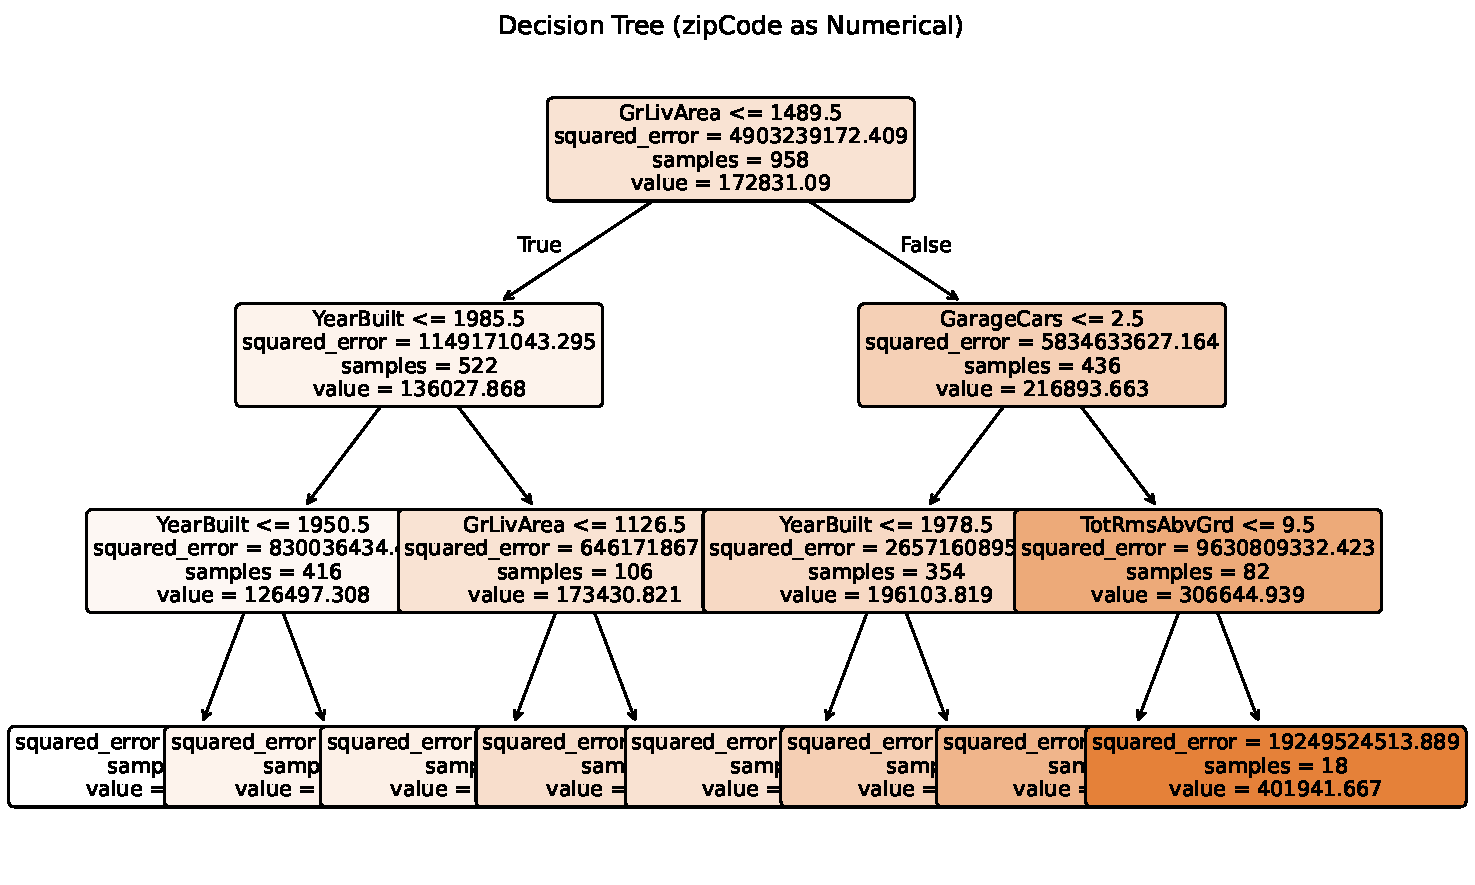
\includegraphics[keepaspectratio]{index_files/figure-pdf/visualize-tree-python-output-1.pdf}}

\subsection{Feature Importance
Analysis}\label{feature-importance-analysis}

\{.panel-tabset\}

\subsubsection{Python}\label{python-2}

\pandocbounded{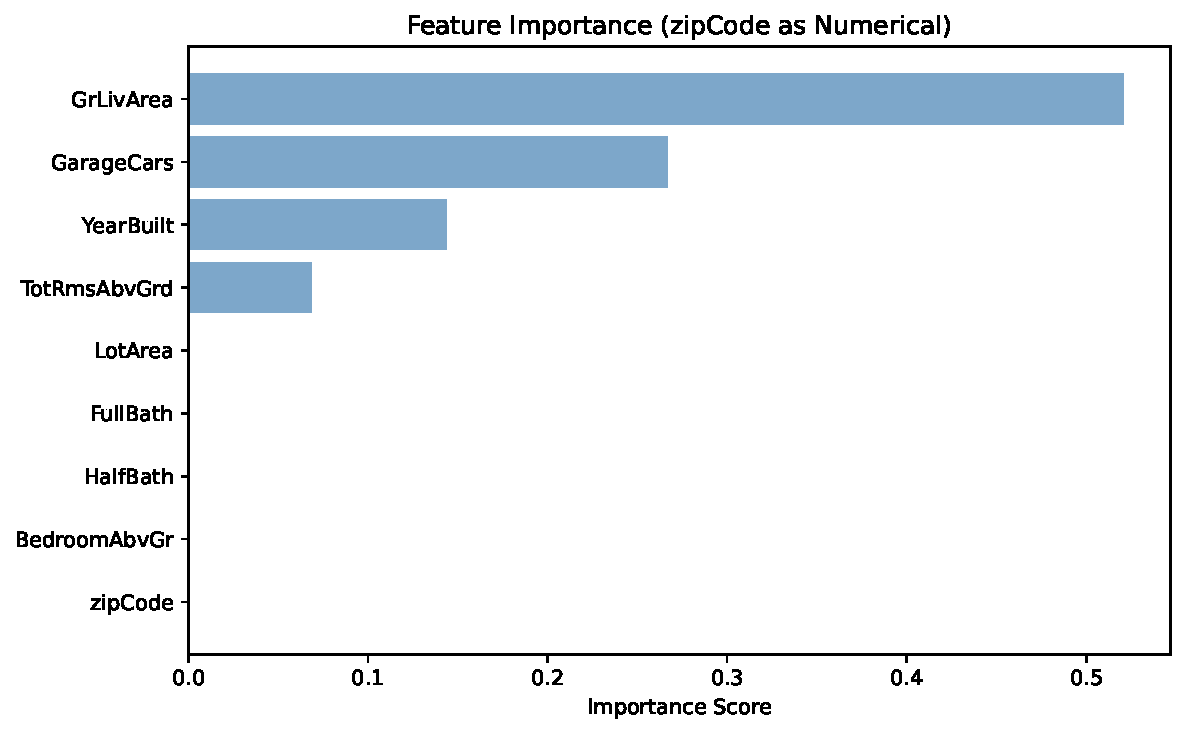
\includegraphics[keepaspectratio]{index_files/figure-pdf/importance-plot-python-output-1.pdf}}

\subsection{Critical Analysis: The Encoding
Problem}\label{critical-analysis-the-encoding-problem}

\{.callout-warning\} \#\# ⚠️ The Problem Revealed

\textbf{What to note:} Our decision tree treated \texttt{zipCode} as a
numerical variable. This leads to zip code being unimportant. Not
surprisingly, because there is no reason to believe allowing splits like
``zipCode \textless{} 50012.5'' should be beneficial for house price
prediction. This false coding of a variable creates several problems:

\begin{enumerate}
\def\labelenumi{\arabic{enumi}.}
\tightlist
\item
  \textbf{Potentially Meaningless Splits:} A zip code of 50013 is not
  ``greater than'' 50012 in any meaningful way for house prices
\item
  \textbf{False Importance:} The algorithm assigns importance to zipCode
  based on numerical splits rather than categorical distinctions OR the
  importance of zip code is completely missed as numerical ordering has
  no inherent relationship to house prices.
\item
  \textbf{Misleading Interpretations:} We might conclude zipCode is not
  important when our intuition tells us it should be important (listen
  to your intuition).
\end{enumerate}

\textbf{The Real Issue:} Zip codes are categorical variables
representing discrete geographic areas. The numerical values have no
inherent order or magnitude relationship to house prices. These must be
modelled as categorical variables.

\subsection{Proper Categorical Encoding: The
Solution}\label{proper-categorical-encoding-the-solution}

Now let's repeat the analysis with zipCode properly encoded as
categorical variables to see the difference.

\textbf{R Approach:} Convert zipCode to a factor (categorical
variable)\\
\textbf{Python Approach:} One-hot encode zipCode (create dummy variables
for each zip code)

\subsubsection{Categorical Encoding
Analysis}\label{categorical-encoding-analysis}

\{.panel-tabset\}

\subsubsection{Python}\label{python-3}

\subsubsection{Tree Visualization: Categorical
zipCode}\label{tree-visualization-categorical-zipcode}

\subsubsection{Python}\label{python-4}

\begin{Shaded}
\begin{Highlighting}[]
\CommentTok{\# Visualize tree with one{-}hot encoded zipCode}
\NormalTok{plt.figure(figsize}\OperatorTok{=}\NormalTok{(}\DecValTok{10}\NormalTok{, }\DecValTok{6}\NormalTok{))}
\NormalTok{plot\_tree(tree\_model\_cat, }
\NormalTok{          feature\_names}\OperatorTok{=}\NormalTok{X\_train\_cat.columns,}
\NormalTok{          filled}\OperatorTok{=}\VariableTok{True}\NormalTok{, }
\NormalTok{          rounded}\OperatorTok{=}\VariableTok{True}\NormalTok{,}
\NormalTok{          fontsize}\OperatorTok{=}\DecValTok{8}\NormalTok{,}
\NormalTok{          max\_depth}\OperatorTok{=}\DecValTok{4}\NormalTok{)}
\NormalTok{plt.title(}\StringTok{"Decision Tree (zipCode One{-}Hot Encoded)"}\NormalTok{)}
\NormalTok{plt.tight\_layout()}
\NormalTok{plt.show()}
\end{Highlighting}
\end{Shaded}

\pandocbounded{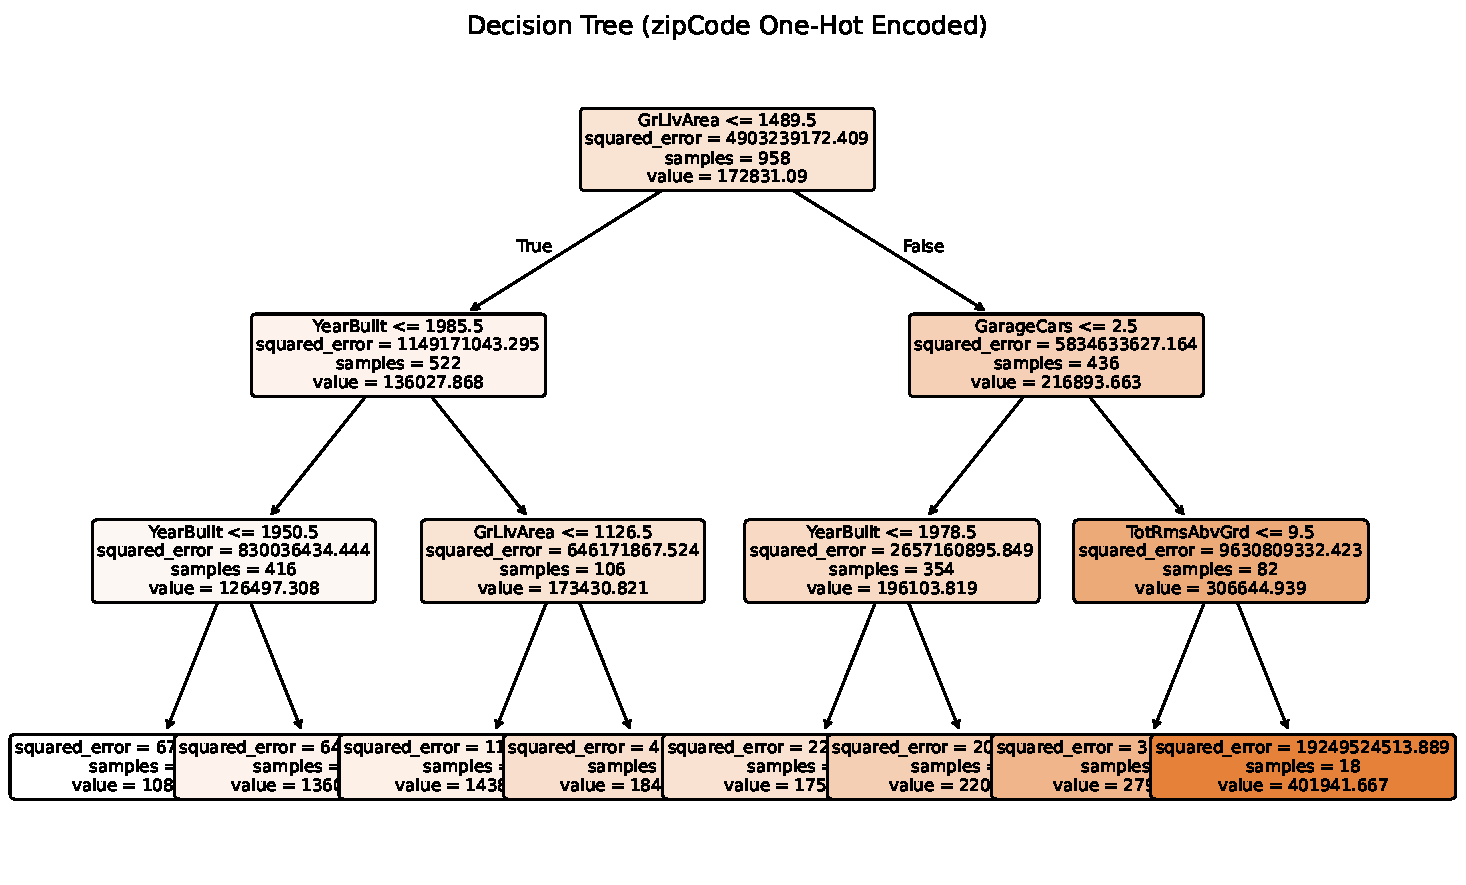
\includegraphics[keepaspectratio]{index_files/figure-pdf/visualize-tree-cat-python-output-1.pdf}}

\subsubsection{Feature Importance: Categorical
zipCode}\label{feature-importance-categorical-zipcode}

\{.panel-tabset\}

\subsubsection{Python}\label{python-5}

\pandocbounded{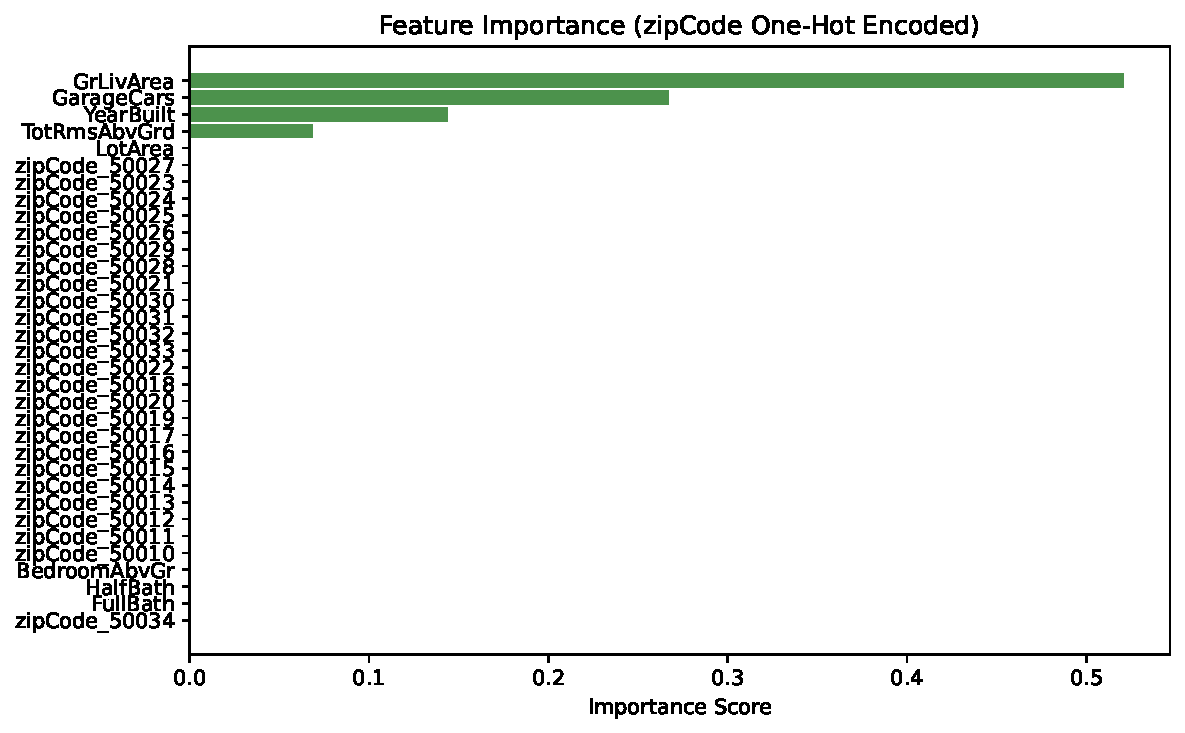
\includegraphics[keepaspectratio]{index_files/figure-pdf/importance-plot-cat-python-output-1.pdf}}

\subsubsection{Question 1\{\#sec-Question 1\}
:}\label{question-1sec-question-1}

Zip Codes should always be modeled as a categorical variable because the
numbers don't mean anything. This isn't something our model understands
and when it is numerical it will most likely misinterpret the data.
Typically it causes the model to view the higher numerical zip code as
more valuable or better than the lower numerical zip code which doesn't
represent the codes correctly. That's why it is important to catagorize
these zip codes, as having a different zip code may affect the price of
a house, but it won't have anything to do with the number. This goes for
all catagorical data, as they need to be properly handled so we can
understand how they affect our model. The model is good at what it does
but anything that it doesn't understand, it will not be able to adapt to
understand it. We have to ensure the input is something the model can
interpret properly and give a good output.

\subsubsection{Question 2 \{\#sec-Question 2\}
:}\label{question-2-sec-question-2}

The language that does a better job modeling after we turn zip code into
a categorical variable is R. The issue we find within python is that,
``However, the scikit-learn implementation does not support categorical
variables for now.'', as taken from the scikit-learn website's user
guide on decision trees. Although Rpart, the function we use in R, does
support this which is why we see the high feature importance of Zip Code
once it becomes a catagorical variable. We can see in python's feature
importance that it just disregards the Zip Code variable giving us a
less accurate model than R. So when running decision tree's, especially
when our data set has categorical variables, we want to use R if
possible to get the best possible model.

\end{tcolorbox}




\end{document}
